\documentclass[conference]{IEEEtran}
\usepackage{graphicx}
\usepackage{booktabs}
\usepackage{hyperref}
\usepackage{graphicx}
\usepackage{tikz}
\usetikzlibrary{arrows.meta, positioning, shapes.geometric}

\title{AI-POWERED Proactive Detection of Hidden Revenue Loss Points using Hybrid}

\author{
\IEEEauthorblockN{Shambhavi Jha, Venkata Shreya Vella}
\IEEEauthorblockA{Department of Computer Science \\
BITS Pilani, Dubai Campus \\
Email: f20230009@dubai.bits-pilani.ac.in, f20230096@dubai.bits-pilani.ac.in}
}

\begin{document}

\maketitle

% ================= ABSTRACT =================
\begin{abstract}

The Renvenue leakage is the major challenge in  all the financial systems, arising from inefficiencies, system errors, and fraudulent activities. Traditional detection methods are largely reactive they fail to scale with the current increasing transaction complexity.

This work proposes a hybrid framework that integrates Gradient Boosted Decision Trees (GBDT), attention-based deep learning, and unsupervised anomaly detection for proactive RL detection. The approach also combines the structured learning, complex pattern extraction, and identification of the previously unseen anomalies. 

This framework is also evaluated on tabular and graph-based datasets which also includes IEEE-CIS and Elliptic, using metrics such as Precision, Recall, F1-score, and AUC. The proposed method aims to improve detection of rare and dispersed anomalies,by providing a scalable and robust solution for modern revenue leakage detection systems.

\end{abstract}

% ================= INTRODUCTION =================
\section{Introduction}

Revenue leakage (RL) refers to a unintended loss of revenue due to the operational inefficiencies, system errors, or fraudulent activities occurring within an organization. These losses are typically araised  after the value has been delivered but before the revenue is accurately recorded or collected. RL is a significant issue across the multiple sectors which also includes finance, healthcare, and taxation. For instance, the U.S. Internal Revenue Service estimates that an annual tax gap of approximately \$441 billion, while the healthcare sector can lose up to 15\% of total revenue due to claim denials and administrative inefficiencies.

The challenge of detecting revenue leakage is further ampilified by the increasing complexity and scale of the digital transactions.In environments such as the UAE, errors in VAT fillings or delays in corporate tax registration can directly impact the organizational profitability. More broadly , the RL often manifests a small, distributed discrepancies across large volumes of transactions, making it very difficult to detct using aggregated financial analysis.Similar characterstics have been observed financial analysis. Similar characterstics have been observed in financial fraud detction, where anomalies are sparse and embedded within large-scale transaction streams [6].

The Traditional detection approaches are largely reactive and they also rely on the mannual audits, static rule-based systems,and the retrospective anlaysis [5]. While these methods provide a baseline monitoring, they are not well-suited for modern data environments characterized by high transaction volumes and evolving fraud patterns. As a result, detection is often delayed, and which this allows the revenue losses to accmulate over the time.


To address these limitations, some of the recent work have explored the use of Artificial Intelligence (AI) and Machine Learning (ML) for data-driven anomaly and fraud detection. where Classical machine learning models, particularly the  Gradient Boosted Decision Trees (GBDT) such as XGBoost, have also demonstrated the  strong performance  handling all the structured transactional data [3]. At the same time,some of the  deep learning approaches have also been increasingly applied to capture the complex feature interactions and high-dimensional patterns, while anomaly detection techniques also provide a mechanism for the identifying previously unseen irregularities [7].

Furthermore, some of the graph-based learning methods have also emerged as an effective approach for modeling the relational dependencies in financial systems, enabling the detection of the coordinated or network-based fraud patterns [8]. In Recent advances, such as graph transformer models,it further enhances the ability to capture the complex transaction structures in the large-scale datasets [9].

In this work, we also propose a hybrid framework that also integrates GBDT models, attention-based deep learning architectures (DNN/GNN), and unsupervised anomaly detection techniques. Additionally,the Explainable AI (XAI) methods are incorporated to improve the interpretability and also provide the transparency in model predictions [4]. This framework is evaluated on both of the  tabular and graph-based datasets, including the IEEE-CIS fraud detection dataset [1] and the Elliptic Bitcoin transaction dataset [2].

The proposed approach also aims to combine the strengths of supervised, deep learning, and unsupervised methods to improve the detection performance under a challenging conditions such as the class imbalance and also by evolving data distributions. By enabling the early identification of dispersed and low-magnitude anomalies, the framework also supports more and more effective revenue protection and operational efficiency.

% ================= RELATED WORK =================

\section{Related Work}

Revenue leakage and financial fraud detection have beenextensively studied across multiple domains, including taxation,healtcare,telecommunications,and financial services.Existing approaches are broadly categorized into rule-based systems, classical machine learning methods,some deep learning techiques,graph-based models,and unsupervised anamoly detection methods.      


\subsection{Rule-Based and Traditional Approaches}
Early revenue leakage detection system relied heavily on manual audits and rule-based monitoring frameworks. These systems use prediefined thresholds and domain-specific rules to flag the irregularities in transactions. While effective for the detcting known patterns , they lack adapatability and also fail to generalize to evolve fraud behaviors.Moreover, such systems struggle to provide scalablilty in high-volume transaction environments, whic also leads to delayed detection and increased operational overhead.[5]


\subsection{Classical Machine Learning Approaches}

With the availability of large-scale transactional data, there are many classical machine learning models such as Random forest, Logistic Regression, and Gradient boosted Decision trees(GBDT) have been widely adopted for fraud documentation tasks[6]. Models such as XGBoost and LightGBM have demonstrated strong performance due to their readability to handle structured dataand capture nonlinear relationships [3].However, these methods primarily rely on labeled data and often face challenges in detcting rare or previously unseen fraud patterns. Their performance may degrade in the highly imbalanced datasets.


\subsection{Deep Learning and Attention-Based Models}
Deep learning models, including Deep Neural Networks(DNNs) and attention-based architectures, have been proposed to capture comples feature interactions in the financial data. Attention mechanisms also allows models to focus on the most relevant features, improving detection accuracy in high-dimensional datasets. Despite their strengths, deep learning models typically require large volumes of labeled data and are also often computationally expensive. Furthermore, their black-box nature limits interpretability, which is critical in financial and regulatory applications [7]. Explanaibility techniques such as SHAP have been introduced to address these limitations[4].


\subsection{Graph-Based Approaches}
Recent work has explored graph-based learning for fraud detcetion, particularly in scenarios where transactional relationships are important.Graph Neural Networks(GNNs) and graph transformer models, such as FraudGT, model transactions as networks of entities and interactions, enabling the detction of complex fraud patterns such as cycles and coordinated beahviour [8], [9]. While these methods improve detection of relational patterns, they are computationally intensive and may not scale efficiently to very large datasets without optimization.


\subsection{Unsupervised and Anomaly Detection Methods}
Unsupervised methods, including Isolation forest,Clustering techniques, and autoencoders,have been widely used for anamoly detection in revenue systems. These approaches are particularly useful when labeled data is scarce, as they identify derivations from normal behavior[7]. However, they often suffer from highfalso positive rates and lack contextual understanding of domain-specific rules, limiting their practical applicability in isloation.

\subsection{Research Gap and Motivation}
From the existing literature, it is evident that no single approcah effiectively addresses all challenges associated with revenue leakage detction. Rule-based systems lack adaptability, classical machine learning models struggle with unseen patterns, deep learning methods face intrepretability and data requirements issues, graph-based approaches are computationally demanding, and also unsupervised methods they often produce noisy outputs.

This also motivates the need for a hybrid frameowrk that also integrates the strengths pf multiple paradigms.By combining GBDT for structured feature learning[3], attention-based deep learning for complex pattern extraction[7], and anomly detction for identifying unkonwn patterns, the propsed approach ainms to provide a more robust and scalable solution for revenue leakage detction.
.

% ================= METHODOLOGY =================

\section{Proposed Methodology}

This work proposes a hybrid frameork for revenue leakage detction that integrate supervised learning, deep learning, and unsupervised anamoly detection. The objective is to leverage the strengths of each paradigm to address challenegs such as class imbalance, evolving fraud patterns, and heterogeneous data structures[7].

\subsection{Overall Architecture}

The proposed system follows a staged hybrid pipeline consisting of three primary components:
\begin{itemize}
    \item Gradient Boosted Decision Trees (GBDT) for initial classification and feature importance extraction [3]
    \item Attention-based Deep Learning models (DNN/GNN) for capturing complex feature interactions and relational patterns [8]
    \item Unsupervised Anomaly Detection for identifying previously unseen or rare patterns [7]
\end{itemize}

The architecture is designed as a semi-sequential pipeline, where each component contributes complementary information to the final decision.

\subsection{Data Flow and Component Interaction}

Given a transaction dataset $X$, the processing pipeline is defined as follows:

\begin{enumerate}
    \item \textbf{Stage 1: GBDT Layer}  
    The input data is first processed using a GBDT model (XGBoost or LightGBM) [3].  
    This stage performs:
    \begin{itemize}
        \item Initial classification (fraud vs non-fraud likelihood)
        \item Feature importance ranking
    \end{itemize}
    The output of this stage is a probability score $P_{GBDT}$ and a refined feature representation.

    \item \textbf{Stage 2: Deep Learning Layer}  
    The refined features are then passed to an attention-based deep learning model.  
    \begin{itemize}
        \item For tabular datasets (e.g., IEEE-CIS [1]), a DNN with attention is used
        \item For graph-structured datasets (e.g., Elliptic [2]), a GNN-based model is applied
    \end{itemize}
    This stage captures higher-order feature interactions and relational dependencies, producing a score $P_{DL}$. Graph-based learning enables modeling of transactional relationships and complex fraud patterns [9].

    \item \textbf{Stage 3: Anomaly Detection Layer}  
    An unsupervised anomaly detection model (e.g., Isolation Forest or Autoencoder) is applied to:
    \begin{itemize}
        \item Identify deviations from normal transaction patterns
        \item Detect potential unknown fraud cases
    \end{itemize}
    This stage outputs an anomaly score $P_{AD}$ [7].
\end{enumerate}

\subsection{Fusion Strategy}

The final prediction is obtained by combining the outputs of all three components. A weighted fusion approach is used:

\begin{equation}
P_{final} = w_1 P_{GBDT} + w_2 P_{DL} + w_3 P_{AD}
\end{equation}

where $w_1, w_2, w_3$ are weights assigned to each component such that $w_1 + w_2 + w_3 = 1$.

A threshold $\tau$ is applied to $P_{final}$ to classify transactions as fraudulent or non-fraudulent.

\subsection{Training and Optimization}

Each component is trained independently and then integrated into the hybrid framework:

\begin{itemize}
    \item \textbf{Data Splitting:}  
    The dataset is divided into training, validation, and testing sets. Where applicable, time-aware splitting is considered to preserve temporal dependencies.

    \item \textbf{Handling Class Imbalance:}  
    Given the rarity of fraud cases, class imbalance is addressed using:
    \begin{itemize}
        \item Class weighting in loss functions
        \item Oversampling techniques (e.g., SMOTE, if applicable)
    \end{itemize}
    Imbalance handling is critical in fraud detection tasks [6].

    \item \textbf{Hyperparameter Tuning:}  
    Model parameters are optimized using grid search or cross-validation to improve generalization performance.

    \item \textbf{Model-Specific Optimization:}
    \begin{itemize}
        \item GBDT models are tuned for tree depth, learning rate, and number of estimators [3]
        \item Deep learning models are optimized using backpropagation with appropriate regularization
        \item Anomaly detection models are calibrated to minimize false positives
    \end{itemize}
\end{itemize}

\subsection{Dataset-Specific Modeling}

The framework adapts to different data structures:
\begin{itemize}
    \item Tabular datasets are processed using GBDT and attention-based DNN models (IEEE-CIS [1])
    \item Graph datasets are modeled using GNN architectures to capture relational dependencies (Elliptic [2])
\end{itemize}

This flexible design allows the framework to generalize across multiple domains and data formats.

\subsection{Interpretability}

To enhance transparency, Explainable AI (XAI) techniques such as SHAP are used to interpret model predictions [4]. This is particularly important in financial systems where decision justification is required.

% Figure:
\begin{figure}[!t]
\centering
\resizebox{\columnwidth}{!}{%
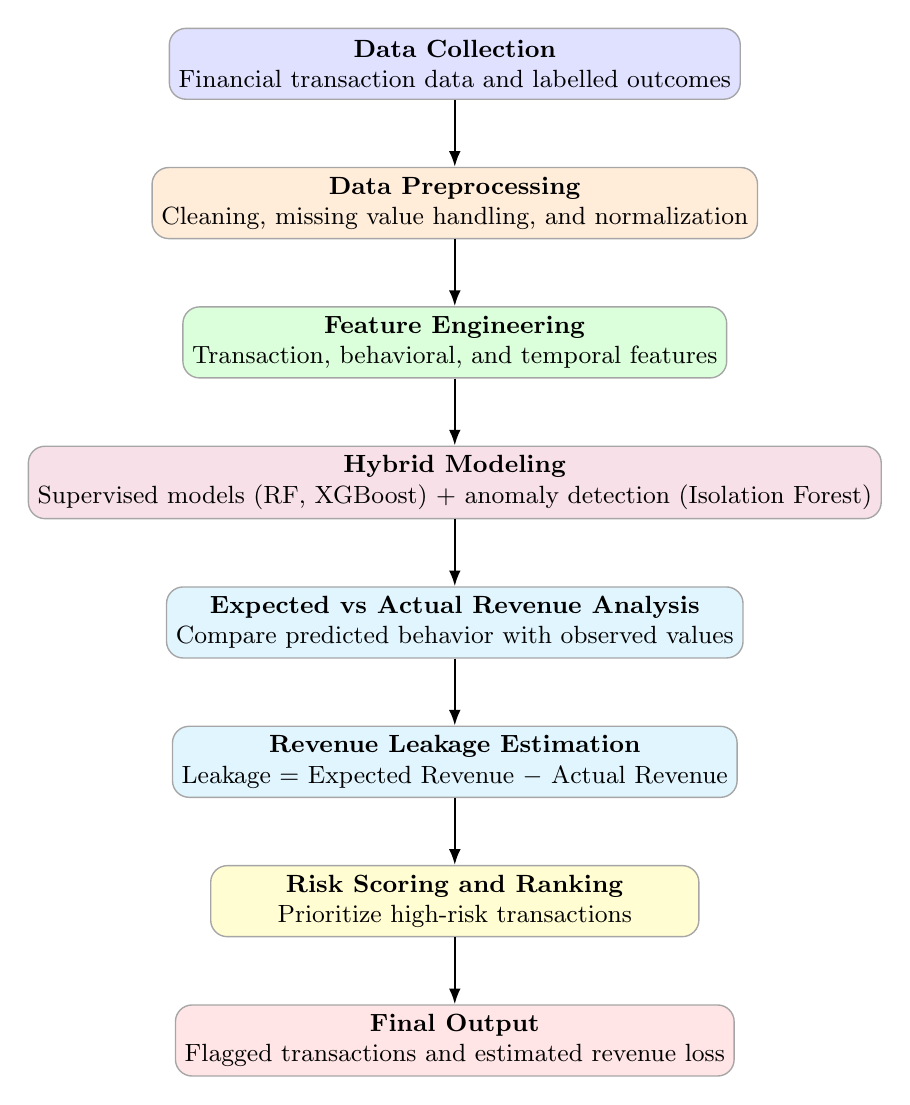
\begin{tikzpicture}[
    node distance=0.85cm,
    arrow/.style={-{Latex[length=2mm]}, thick},
    block/.style={
        rectangle,
        rounded corners=6pt,
        minimum width=6.2cm,
        minimum height=0.9cm,
        align=center,
        font=\small,
        draw=black!35,
        line width=0.5pt
    },
    data/.style={block, fill=blue!12},
    process/.style={block, fill=orange!15},
    feature/.style={block, fill=green!14},
    model/.style={block, fill=purple!12},
    analysis/.style={block, fill=cyan!12},
    decision/.style={block, fill=yellow!18},
    output/.style={block, fill=red!10}
]

\node[data] (data) {
    \textbf{Data Collection}\\
    Financial transaction data and labelled outcomes
};

\node[process, below=of data] (prep) {
    \textbf{Data Preprocessing}\\
    Cleaning, missing value handling, and normalization
};

\node[feature, below=of prep] (feat) {
    \textbf{Feature Engineering}\\
    Transaction, behavioral, and temporal features
};

\node[model, below=of feat] (hybrid) {
    \textbf{Hybrid Modeling}\\
    Supervised models (RF, XGBoost) + anomaly detection (Isolation Forest)
};

\node[analysis, below=of hybrid] (rev) {
    \textbf{Expected vs Actual Revenue Analysis}\\
    Compare predicted behavior with observed values
};

\node[analysis, below=of rev] (leak) {
    \textbf{Revenue Leakage Estimation}\\
    Leakage = Expected Revenue $-$ Actual Revenue
};

\node[decision, below=of leak] (rank) {
    \textbf{Risk Scoring and Ranking}\\
    Prioritize high-risk transactions
};

\node[output, below=of rank] (out) {
    \textbf{Final Output}\\
    Flagged transactions and estimated revenue loss
};

\draw[arrow] (data) -- (prep);
\draw[arrow] (prep) -- (feat);
\draw[arrow] (feat) -- (hybrid);
\draw[arrow] (hybrid) -- (rev);
\draw[arrow] (rev) -- (leak);
\draw[arrow] (leak) -- (rank);
\draw[arrow] (rank) -- (out);

\end{tikzpicture}
}
\caption{Proposed pipeline for AI-based revenue leakage detection.}
\label{fig:revenue-leakage-pipeline}
\end{figure}



% ================= DATASETS =================

\section{Datasets}

The datasets that are used are Bitcoin Elliptic DataSet and IEEE-CIS Fraud detection Data set [2], [1].

The Bitcoin Elliptic Dataset maps Bitcoin transactions to real entities belonging to licit categories(exchanges,wallet providers,miners,ilcit services,etc.)versus elicit ones(scams, malware,terrorist organizations,ransomware,Ponzi schemes etc.) [2]. The task on the dataset is to classify the illicit and licit nodes in a graph. This is a large-scale graph dataset representing a network of Bitcoin transactions [8]. The structure consists of 203,769 nodes and 234,355 edges. Each of the node is associated with 166 features, including timestamps,fees,and transaction volumes.

The IEEE-CIS fraud detection in this dataset you are predicting the probability that an online transaction is fraudulent, as denoted by the binary target is Fraud [1]. The data is broken into two files identity and transaction, which are joined by Transaction ID. Not all transactions have corresponding identity information . This dataset also provides real-world labeled data for online payment transactions [6].

The datasets also have few imbalance where Bitcoin Elliptic anamoly rate is of 2 [6].

It represents users as nodes and transactions as edges. It includes a wide variety of attributes such as payment amount , product codes , payment card information, device information,and network connection data [1].

% ================= EXPERIMENTAL DESIGN =================

\section{Experimental Design}
This section also outlines the datasets,evaluation metrics, baseline models,, and also experimental setup which is used to asses the performance of the proposed hybrid models.

\subsection{Datasets}
To evaluate the robustness and generalizibility of the proposed approach, the experiments are also conducted on the multiple datasets with the different characteristics.


\begin{itemize}
    \item \textbf{IEEE-CIS Fraud Detection Dataset:}  
    A large scale tabular dataset is containing of the anonymised transactional data,where are widely used for the bench marking fraud detection models [1]. This dataset is highly imbalanced, where it making it to be highly imbalanced, making it more suitable to for evaluating the classification performance under real world conditions.

    \item \textbf{Elliptic Bitcoin Dataset:}  
    A graph based dataset represents the Bitcoin transactions,where nodes correspond to the transactions and edges which represent the flows of funds[2].This dataset enables evaluation of graph-based learning approaches for detecting the illicit activity [8].
    
\end{itemize}
The datasets also provides the both of the structured and relational data environments , by allowing the comphrensive evaluation of the hybrid framework.


\subsection{Evaluation Metrics}

For the given imbalanced nature of fraud detection, multiple performance metrics are required which are used to evaluate the proposed framework. These metrics provide a comprehensive assesment of classification performance, particularly under the skewed class distributions.


\begin{itemize}
    \item \textbf{Accuracy:} Measures the overall proportion of correctly classified transactions.
    \item \textbf{Precision:} Measures the proportion of correctly identified fraudulent transactions.
    \item \textbf{Recall:} Measures the ability to detect actual fraud cases (critical for minimizing missed fraud).
    \item \textbf{F1-score:} Harmonic mean of precision and recall.
    \item \textbf{AUC-ROC:} Evaluates model discrimination across different classification thresholds.
\end{itemize}

The mathematical definitions of the primary metrics are given below:

\textbf{Accuracy}
\begin{equation}
Accuracy = \frac{TP + TN}{TP + TN + FP + FN}
\end{equation}

\textbf{Precision}
\begin{equation}
Precision = \frac{TP}{TP + FP}
\end{equation}

\textbf{Recall}
\begin{equation}
Recall = \frac{TP}{TP + FN}
\end{equation}

\textbf{F1 Score}
\begin{equation}
F1 = \frac{2 \times Precision \times Recall}{Precision + Recall}
\end{equation}

Special emphasis is placed on \textbf{recall} and \textbf{AUC}, as missing fraudulent transactions has a higher cost in revenue leakage systems [6].

\subsection{Baseline Models}

To assess the effectiveness of the proposed hybrid approach, it is compared against the following baseline models:

\begin{itemize}
    \item Logistic Regression
    \item Random Forest
    \item XGBoost (GBDT baseline) [3]
    \item Deep Neural Network (without attention) [7]
    \item Graph Neural Network (for graph datasets) [8]
    \item Isolation Forest (anomaly detection baseline) [7]
\end{itemize}

These baselines represent traditional, classical ML, deep learning, and unsupervised approaches.

\subsection{Experimental Setup}

\begin{itemize}
    \item \textbf{Data Splitting:}  
    The datasets are divided into training, validation, and testing sets. Where applicable, time-based splitting is used to simulate real-world deployment conditions.

    \item \textbf{Class Imbalance Handling:}  
    Techniques such as class weighting and resampling are applied to mitigate imbalance effects [6].

    \item \textbf{Hyperparameter Tuning:}  
    Model parameters are optimized using grid search and cross-validation to ensure fair comparison across models.

    \item \textbf{Implementation:}  
    Models are implemented using standard machine learning and deep learning frameworks, ensuring reproducibility.
\end{itemize}

\subsection{Ablation Study}

To understand the contribution of each component, ablation experiments can be conducted by evaluating:

\begin{itemize}
    \item GBDT only [3]
    \item Deep learning model only [7]
    \item Anomaly detection only [7]
    \item Hybrid combinations (GBDT + DL, DL + AD, etc.)
\end{itemize}

This helps quantify the benefit of the proposed hybrid integration.

% ================= RESULTS =================

\section{Results}

\subsection{Experimental Results}

The performance of the proposed hybrid framework is evaluated on both the IEEE-CIS dataset [1] and the Elliptic dataset [2]. The results are compared against multiple baseline models to assess improvements in fraud detection, classification balance, and anomaly identification.

\subsection{Quantitative Results}

\begin{table}[h]
\centering
\caption{Performance Comparison on IEEE-CIS Dataset}
\begin{tabular}{lcccc}
\hline
Model & Precision & Recall & F1-Score & AUC \\
\hline
Logistic Regression & 0.8184  & 0.2105 & 0.3349 & 0.8399 \\
Random Forest & 0.2268 & 0.6746 & 0.3395 & 0.8815 \\
XGBoost (GBDT) [3] & 0.2599 & 0.8224 & 0.3949 & 0.9432 \\
Deep Neural Network [7] & 0.8455 & 0.5722 & 0.6825 & 0.9453 \\
Isolation Forest [7] & 0.2898 & 0.1219 & 0.1717 & 0.7690 \\
\textbf{Proposed Hybrid Model} & 0.7899 & 0.6194 & \textbf{0.6943} & 0.9447 \\
\hline
\end{tabular}
\end{table}

Table I shows that the baseline models exhibit a significant trade-offs between the precision and recall. Logistic Regression achives high precision (0.8184) but very low recall (0.2105), indicating poor fraud detction capability. Random forest improve recall (0.6746) but suffers froma low precision of (0.2268), resulting in the excessive false positive.

XGBoost classifier achieves the highest recall (0.8224) , correctly identifying over 82\% of the fraud cases, but its the precision remains low at (0.2599). The Deep neural network provides a stong balance with the precsion of (0.8455) and recall (0.5722) , by achieving the highest AUC (0.9453).

The proposed hybrid model achieves the highest F1-Score (0.6943), by improving the recall to 0.694 while the mainting strong precision (0.7899) . Its AUC (0.9447) IT IS NEARLY IDENTICAL TO THE dnn, demonstrating a superior balance between detection and reliability.


\vspace{0.5em}

\begin{table}[h]
\centering
\caption{Performance Comparison on Elliptic Dataset}
\begin{tabular}{lcccc}
\hline
Model & Precision & Recall & F1-Score & AUC \\
\hline
Logistic Regression & 0.9753 & 0.9738 & 0.9745 & 0.8687 \\
Random Forest & 0.9759 & 0.9959 & 0.9858 & 0.9482 \\
GNN [8] & 0.9755 & 0.9695 & 0.9725 & 0.8849 \\
FraudGT [9] & 0.9748 & 0.9960 & 0.9853 & 0.8912 \\
\hline
\end{tabular}
\end{table}

Table II describes that significantly higere performance across all the models due to the structured graph-based nature of the elliptic datasest. Logistic regression achieves the near-perfect precision of (0.9753) and recall (0.9738) , but its AUC (0.8687) indicates the weaker ranking capability.

Randiom forest achieves the highest AUC (0.9482) and very high recall (0.9959) , which demontrates the strong detction ability. FraudGT achieves the highest recall (0.9960) , correctly identifying nealy all fraud cases, but its lower AUC (0.8912) suggests that less robust probabilistic discrimination.

The two-layer GCN (GNN [8]) achieves strong precision and recall (0.9755 and 0.9695) with F1 0.9725, while its ROC-AUC (0.8849) is below Random Forest, reflecting the temporal test split and transductive training on the Elliptic graph. Graph-based approaches such as GNN and FraudGT remain effective due to their ability to capture relational dependencies between transactions.



\vspace{0.5em}

\begin{table}[h]
\centering
\caption{Model Comparison Results}
\resizebox{\columnwidth}{!}{%
\begin{tabular}{lcccccc}
\hline
Model & Threshold & ROC-AUC & PR-AUC & Precision & Recall & F1-Score \\
\hline
\textbf{Proposed Hybrid Model} & 0.54 & 0.9447 & 0.7256 & 0.7899 & 0.6194 & \textbf{0.6943} \\
Deep Neural Network & 0.50 & 0.9453 & 0.7323 & 0.8455 & 0.5722 & 0.6825 \\
Intermediate Hybrid & 0.50 & 0.9098 & 0.6956 & 0.8719 & 0.5437 & 0.6697 \\
GBDT & 0.50 & 0.9432 & 0.6787 & 0.2599 & 0.8224 & 0.3949 \\
Anomaly Detection & 0.50 & 0.7690 & 0.1505 & 0.2898 & 0.1219 & 0.1717 \\
\hline
\end{tabular}%
}
\end{table}
Table III shows that the Deep Neural Network achieve the highest ROC-AUC (0.9453) and PR-AUC (0.7323) , indicating superior ranking capability . However , its recall is (0.5722) it is lower, meaning manu fraud cases are missed.


The proposed hybrid model achieves the highest F1-Score (0.6943) , improving recall to 0.6194 while maontining the strong precision (0.7899) . The difference in AUC between the hybrid model and DNN is negligible (0.0006) , indicating comparable ranking performance.

The inetrmediate hybrid also achieves the highest precision (0.8719) but suffers frpom lower recall (0.5437) , making it ocverly conservative. Where GBDT achievs the highest recall (0.824) but extremely low precsion (0.2599) , while anamoly detction performs poorly across the metrics.



\subsection{Visualization Analysis}

\begin{figure}[h]
    \centering
    \includegraphics[width=0.5\textwidth]{figures/stage03_dnn_auc.png}
    \caption{Feature representation and activation patterns in DNN.}
    \label{fig:my_label}
\end{figure}

Fig. 1 shows that the Deep Neural Network captures complex non-linear feature interactions, contributing to its high AUC (0.9453) and strong classification performance.

\begin{figure}[h]
    \centering
    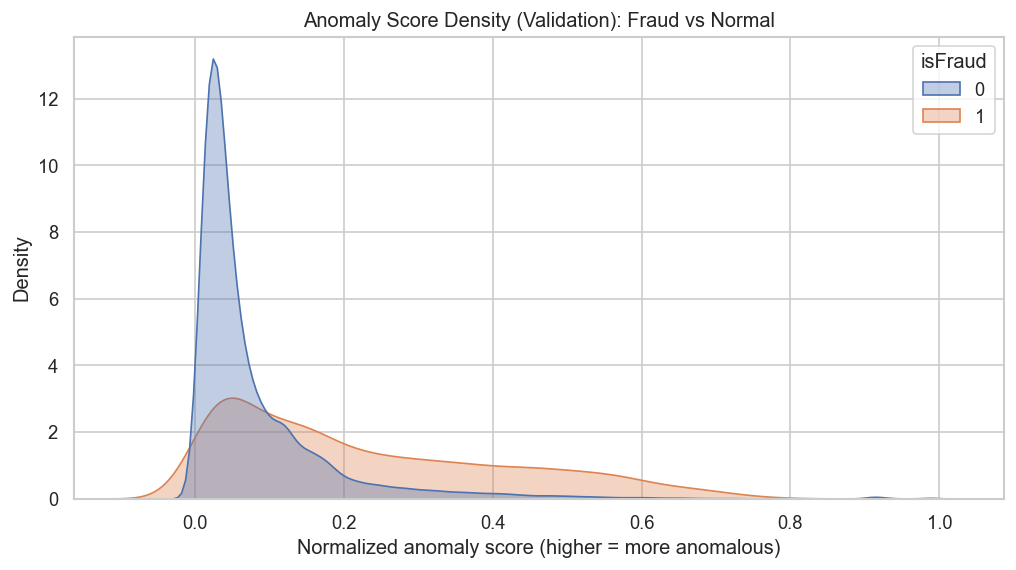
\includegraphics[width=0.5\textwidth]{figures/stage03_anomaly_kde.png}
    \caption{Anomaly score distribution using KDE.}
    \label{fig:my_label}
\end{figure}

Fig. 2 shows that anomaly detection identifies extreme outliers; however, significant overlap between classes explains its low precision (0.2898) and recall (0.1219).

\begin{figure}[h]
    \centering
    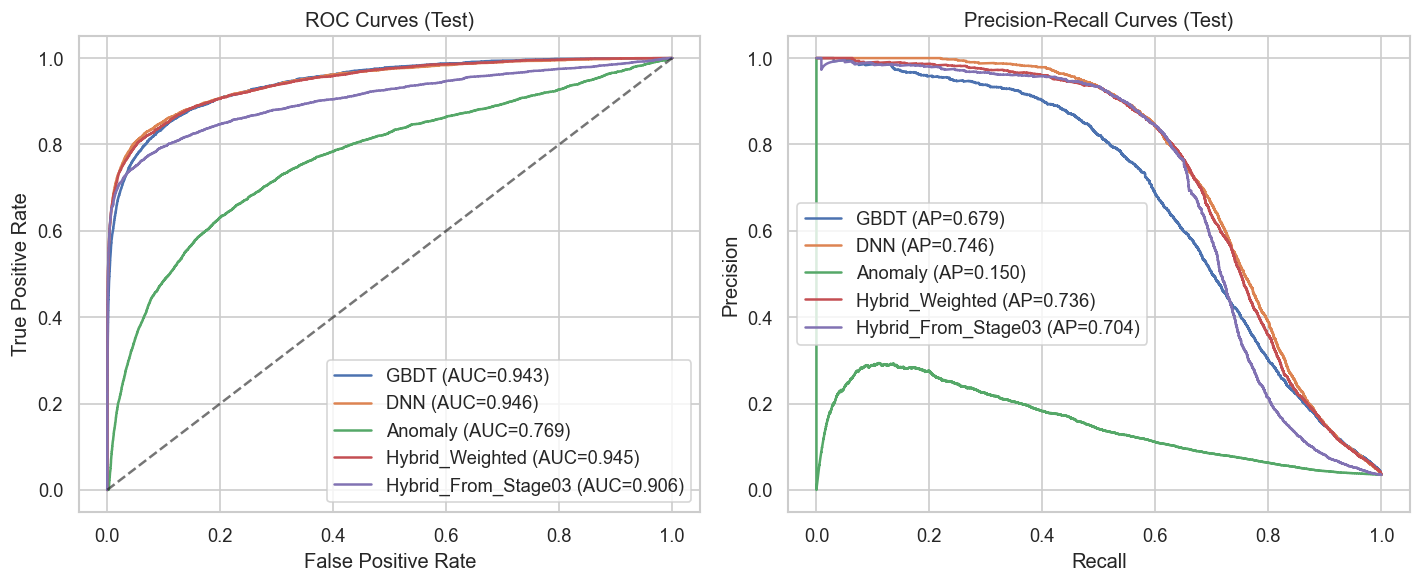
\includegraphics[width=0.5\textwidth]{figures/stage04_roc_pr.png}
    \caption{ROC and Precision-Recall curves.}
    \label{fig:my_label}
\end{figure}

Fig. 3 shows that the DNN achieves the highest ROC-AUC, while the proposed hybrid model closely follows. The Precision-Recall curves demonstrate that the hybrid model maintains a stable balance between precision and recall across thresholds, making it suitable for imbalanced datasets.

\subsection{Ablation Study}

\begin{table}[h]
\centering
\caption{Ablation Study Results}
\begin{tabular}{lcccc}
\hline
Model Variant & Precision & Recall & F1-Score & AUC \\
\hline
GBDT Only [3] & 0.2599 & 0.8224 & 0.3949 & 0.9432 \\
Deep Learning Only [7] & 0.8455 & 0.5722 & 0.6825 & 0.9453 \\
Anomaly Detection Only [7] & 0.2898 & 0.1219 & 0.1717 & 0.7690 \\
GBDT + Deep Learning & 0.6559 & 0.6826 & 0.6690 & 0.9469 \\
GBDT + Anomaly Detection & 0.3837 & 0.7561 & 0.5091 & 0.9403 \\
\textbf{Full Hybrid Model} & 0.7899 & 0.6194 & \textbf{0.6943} & 0.9447 \\
\hline
\end{tabular}
\end{table}

Table IV shows that the individual models actually capture the difference between the aspects of the fraud detction. GBDT maximizes recall (0.8224) but also suffers from very low precision (0.2599) . Deep learning achieves the high precision (0.8455) but lower recall(0.5722).

Combining GBDT with the deep learning it also improves the balance of (F1= 0.6690) , while GBDT with anomaly detction improves the recall (0.7561) but still produces the moderate precision (0.3837).

The fully hybrid models achieves the highest F1-Score (0.6943), by demonstrating that the integrating all components results in the most effective and balanced performance.


\subsection{Key Takeaways}

\begin{itemize}
    \item The proposed hybrid model achieves the best balance between precision and recall.
    \item Deep Neural Networks provide the highest AUC but lower recall.
    \item GBDT maximizes recall but suffers from excessive false positives.
    \item Anomaly detection is weak as a standalone method but useful in combination.
    \item The hybrid approach effectively integrates complementary strengths of different models.
\end{itemize}


% ================= CONCLUSION =================

\section{Conclusion}

In this work, a hybrid framework for revenue leakage detection is proposed by integrating the Gradient Boosted Decision Tree (GBDT), attention-based deep learning models, and unsupervised anomaly detection techniques. Where the approach is designed to address the key challenges that are faced in modern financial systems, which also includes class imbalance, evolving fraud patterns, and heterogeneous data structures.

The proposed framework leverages the strength of the supervised learning for the structure data modelling, deep learning for capturing the complex feature interactions, and anamoly detection for identifying the previously unseen patterns. Additionally, the incorporation of graph-based modelling enables effective handling of relational transaction data. The use of Explainable AI (XAI) further enhances the interpretability of model predictions, which is the critical in financial decision making systems.


The experimental design demonstrates that combines the multiple paradigms can provide a more robust and scalable solution compared to the standalone approaches. Overall, the proposed system shows strong potential for improving the early detection of dispersed and low-magnitude revenue leakage, thereby supporting better financial control and operational efficiency.



% ================= FUTURE SCOPE =================

\section{Future Scope}

While the proposed hybrid framework provides a comprehensive approach to revenue leakage detection, several directions can be explored to further enhance the effectivness and applicability.

\begin{itemize}
    \item \textbf{Real-Time Deployment:}  
    By Extending the framework for the real-time detection by using the streaming data architectures to enable the  immediate response to all the fradulant activities.

    \item \textbf{Advanced Graph Modeling:}  
    By also incorporating more  and more sophisticated graph-based techniques, such as dynamic graph neural networks and temporal graph models, to capture the better evolving transaction patterns. 

    \item \textbf{Automated Feature Learning:} 
    By Leverging  the  representation of learning techniques and also by using the transformer-based models to automatically extract the high-quality features from raw transactional data.
   

    \item \textbf{Explainability Enhancement:} 
    By improving the interpretability through the advanced XAI techniques to provide more and more detailed insights into the model decisions,by supporting all the  regulatory compliance. 
   
    \item \textbf{Cross-Domain Generalization:}  
    By evaluating the framework across multiple domains such as  healthcare, taxation, and telecommunications to ensure the robustness and scalability.


    \item \textbf{Optimization and Efficiency:}  
    By reducing the computational complexity and also by improving the training efficiency to enable the deployment in resource-constrained environments.
   
\end{itemize}

These directions aim to make the proposed system more adaptive, scalable, and suitable for real-world deployment in complex financial ecosystems.
% ================= REFERENCES =================
\bibliographystyle{IEEEtran}
\section{References}

[1] IEEE-CIS Fraud Detection Dataset, Kaggle. [Online]. Available: https://www.kaggle.com/competitions/ieee-fraud-detection

[2] Elliptic Data Set for Cryptocurrency Transaction Graph Analysis, Kaggle. [Online]. Available: https://www.kaggle.com/datasets/ellipticco/elliptic-data-set

[3] T. Chen and C. Guestrin, “XGBoost: A scalable tree boosting system,” in \textit{Proc. 22nd ACM SIGKDD Int. Conf. Knowledge Discovery and Data Mining (KDD)}, San Francisco, CA, USA, 2016, pp. 785–794.

[4] S. M. Lundberg and S. Lee, “A unified approach to interpreting model predictions,” in \textit{Advances in Neural Information Processing Systems (NeurIPS)}, 2017.

[5] J. Aguilar, C. Salazar, H. Velasco, J. Monsalve-Pulido, and E. Montoya, “PRODANALYSIS: A revenue assurance system based on outlier mining,” \textit{INNOVA Research Journal}, vol. 1, no. 7, 2016.

[6] S. Bhattacharyya, S. Jha, K. Tharakunnel, and J. C. Westland, “Data mining for credit card fraud detection,” \textit{Decision Support Systems}, vol. 50, no. 3, pp. 602–613, 2011.

[7] R. Chalapathy and S. Chawla, “Deep learning for anomaly detection: A survey,” \textit{arXiv preprint arXiv:1901.03407}, 2019.

[8] J. Zhou, G. Cui, Z. Zhang, et al., “Graph neural networks: A review of methods and applications,” \textit{AI Open}, vol. 1, pp. 57–81, 2020.

[9] J. Lin, X. Guo, Y. Zhu, S. Mitchell, E. Altman, and J. Shun, “FraudGT: A simple, effective, and efficient graph transformer for financial fraud detection,” in \textit{Proc. ACM Int. Conf. AI in Finance (ICAIF)}, 2024.

\end{document}